\documentclass[a4paper,10pt]{article}
\usepackage[utf8]{inputenc}
\usepackage{graphicx}
%\usepackage{subfigure}
%\usepackage{a4wide}
\usepackage{fancyhdr}
\usepackage{algorithm}
\usepackage{algorithmic}
\usepackage{tikz}
\usepackage{empheq}
\usetikzlibrary{trees}
%\usepackage{multirow}
\usepackage{amssymb,amsmath}
\usepackage{amsthm,amsfonts}
\usepackage{float}
\graphicspath{ {images/} }
\usepackage{listings}
\usepackage{color}

\pagestyle{fancy}
\renewcommand{\headrulewidth}{0.1pt}
\renewcommand{\footrulewidth}{0.1pt}
\setlength{\parindent}{0cm}
\documentclass[parskip=full]{scrartcl}
\usepackage{subcaption}
\captionsetup{compatibility=false}

\definecolor{mygreen}{rgb}{0,0.6,0}
\definecolor{mygray}{rgb}{0.5,0.5,0.5}
\definecolor{mymauve}{rgb}{0.58,0,0.82}
\lstset{ %
  backgroundcolor=\color{white},   % choose the background color; you must add \usepackage{color} or \usepackage{xcolor}
  basicstyle=\footnotesize,        % the size of the fonts that are used for the code
  breakatwhitespace=false,         % sets if automatic breaks should only happen at whitespace
  breaklines=true,                 % sets automatic line breaking
  columns=flexible,
  captionpos=b,                    % sets the caption-position to bottom
  commentstyle=\color{mygreen},    % comment style
  %deletekeywords={...},           % if you want to delete keywords from the given language
  %escapeinside={\%*}{*)},         % if you want to add LaTeX within your code
  extendedchars=true,              % lets you use non-ASCII characters; for 8-bits encodings only, does not work with UTF-8
  frame=none,	               % adds a frame around the code
  keepspaces=true,                 % keeps spaces in text, useful for keeping indentation of code (possibly needs columns=flexible)
  keywordstyle=\color{blue},       % keyword style
  language=C,                   % the language of the code
  %otherkeywords={*,...},          % if you want to add more keywords to the set
  numbers=letf,                    % where to put the line-numbers; possible values are (none, left, right)
  numbersep=10pt,                  % how far the line-numbers are from the code
  numberstyle=\tiny\color{mygray}, % the style that is used for the line-numbers
  %rulecolor=\color{black},        % if not set, the frame-color may be changed on line-breaks within not-black text (e.g. comments (green here))
  showspaces=false,                % show spaces everywhere adding particular underscores; it overrides 'showstringspaces'
  showstringspaces=false,          % underline spaces within strings only
  showtabs=false,                  % show tabs within strings adding particular underscores
  stepnumber=1,                    % the step between two line-numbers. If it's 1, each line will be numbered
  stringstyle=\color{mymauve},     % string literal style
  tabsize=4,	                   % sets default tabsize to 2 spaces
  %title=\lstname                  % show the filename of files included with \lstinputlisting; also try caption instead of title
  xleftmargin=1cm
}



\usepackage{advdate}

\newcommand{\advanceday}[1][1]{%O segundo parâmetro define a quantidade de dias adiante
\begingroup
\AdvanceDate[#1]%
\today%
\endgroup
}%



% ---------- DEFINIÇÕES PARA CAPA E CONFIGURAÇÕES DE CABEÇALHO E RODAPÉ

\def \materia {Introdução à Programação Paralela}
\def \semestre {2017/02}
\def \city {Belo Horizonte}
\def \numeropratica {Parte 01}
\def \authora {Gustavo Borba}
\def \authors { \authora }
\def \praticano {Trabalho Prático \numeropratica}
\def \titulopratica {Melhora de Perfórmance em uma Multiplicação de Matrizes simples}




% ---------- CABEÇALHOS E RODAPÉS

\lhead{ \praticano }
\rhead{ \thepage } 
\lfoot{ \authors }
\rfoot{ \today }
\cfoot{}




\begin{document}


% ---------- CAPA

\thispagestyle{empty}


\begin{center}

    \begin{minipage}[l]{10cm}{
        \begin{center}
            \materia \\ \semestre \\
        \end{center}
    }
    \end{minipage}
     
    \vfill
     
    \begin{minipage}[l]{11cm}{
       \begin{center}
       \Large{ \praticano:  \\ \titulopratica }
       \end{center}
    }
    \end{minipage}

\end{center}


\vspace*{8cm}

\begin{center}
    \begin{minipage}[l]{10cm}{
    \center \authora \\ \city, \today \\
 }
 \end{minipage}
 \end{center}

\newpage
%\thispagestyle{empty}

\newpage
\clearpage
\setcounter{page}{1}


% ----------  Início do Relatório


\section{Introdução}

O presente trabalho tem o objetivo de, em sua primeira etapa, experimentar otimizações de código em um algoritmo de multiplicação de matrizes, de forma a melhorar a performance do mesmo em observancia à plataforma que será executado. Ao final desta etapa, espera-se que o código tenha um desempenho melhor, comparado ao seu original, e que esteja mais fácil de implementar sua paralelização. 

\section{Metodologia}

De acordo com orientações descritas por BILMES\cite{bilmes}, o código de duas das três implementações disponibilizadas foi alterado para explicitar características que podem ser utilizadas pelo otimizador do compilador. \\

Os arquivos com os códigos originais foram mantidos, para fins de comparação com os algoritmos alterados. Para estes últimos, uma nova linha no makefile foi criada para cada um, e na pasta do projeto pode-se verificar a presença do sufixo \textit{borba-}, indicando uma versão alterada do arquivo. \\






\subsection{Remover explicitamente falsas dependências}

Para garantir a corretude das operações, os compiladores não assumem que, ao acessar um ponteiro que já fora acessado anteriormente, os mesmos dados estarão lá (afinal de contas, outra função pode ter acesso a esse ponteiro e alterar seu valor), de modo que as operações sobre ponteiros exigem, em sua maioria, acessos constantes à memória. 

Como o programa em questão trata de três matrizes distintas, nenhuma das matrizes será alterada por uma função externa durante a execução das multiplicações. Dessa forma, é possível adicionar a cláusula \textbf{restrict} aos ponteiros recebidos pela função, que indica que apenas aqueles ponteiros ou valores diretamente derivados dele serão utilizados para acessar aquela área de memória. 

\begin{lstlisting}
void square_dgemm (int n, 
                double* restrict A, double* restrict B, double* restrict C)
\end{lstlisting}

O compilador saberá, dessa forma, que não é necessário realizar um fetch dos dados, à menos que haja um cache miss, pois apenas aquele ponteiro referencia a matriz em questão.


\subsection{Explorando melhor os Registradores}


Realizando o profiling do código original com a ferramenta \textbf{perf}, verifica-se que o tempo de acesso à memória é o principal gargalo do programa em questão. Ao verificar os \textit{misses}, obtemos um resultado como o apresentado na Figura \ref{fig:perf_mem}, ficam evidentes dois eventos onde se têm um custo de performance elevado


\begin{figure}[H]
    \begin{center} 
        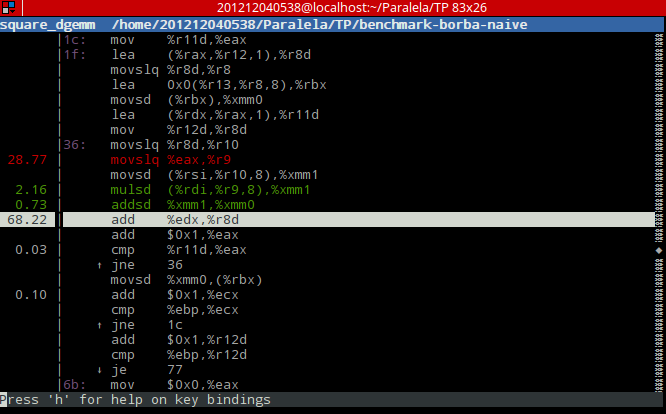
\includegraphics[scale=0.5]{images/perf_mem}
    \end{center}
    \caption{Profiling realizado pelo programa perf no algoritmo de multiplicação de matrizes ingênuo, em termos de \textit{misses} totais. Percebe-se duas instruções com maior custo em performance }
    \label{fig:perf_mem}
\end{figure}

Analisando o código exibido, percebe-se que  partes mais onerosas em termos de memória são um load e uma soma, cujo armazenamento se dá em endereço de memória.

\begin{lstlisting}
void square_dgemm (int n, double* A, double* B, double* C){
  for (int i = 0; i < n; ++i)
    for (int j = 0; j < n; ++j){}
      C[i+j*n] = C[i+j*n]; // aqui
      for( int k = 0; k < n; k++ )
        C[i+j*n] += A[i+k*n] * B[k+j*n]; // aqui
    }
}
\end{lstlisting}

Para reduzir essa demanda por acessos à memória, transforma-se o ponteiro em uma variável local. Como trata-se de um valor muito utilizado, inclusive, a utilização da cláusua \textbf{register} é ainda mais eficiente. Assim, por completo, o código ingênuo se torna o seguinte:


\begin{lstlisting}
void square_dgemm (int n, double* restrict A, double* restrict B, double* restrict C) {
  for (int i = 0; i < n; ++i)
    for (int j = 0; j < n; ++j) {
      int jn = j*n;
      register double cij = C[i+jn];
      for( int k = 0; k < n; k++ ){
        double Aikn=A[i+k*n];
        double Bkjn=B[k+jn];
        cij += Aikn * Bkjn;
      }
      C[i+jn] = cij;
    }
}
\end{lstlisting}

repetindo o processo com a ferramenta \textbf{perf}, mas agora com tempo de CPU, verifica-se na Figura \ref{fig:perf_ops} que o gargalo de processamento ainda ocorre nestas duas operações, sendo dispensável a criação de mais variáveis temporárias para a otimização de índices, por exemplo, pois estes são pouco utilizados com relação aos anteriormente citados.



\begin{figure}[H]
    \begin{center} 
        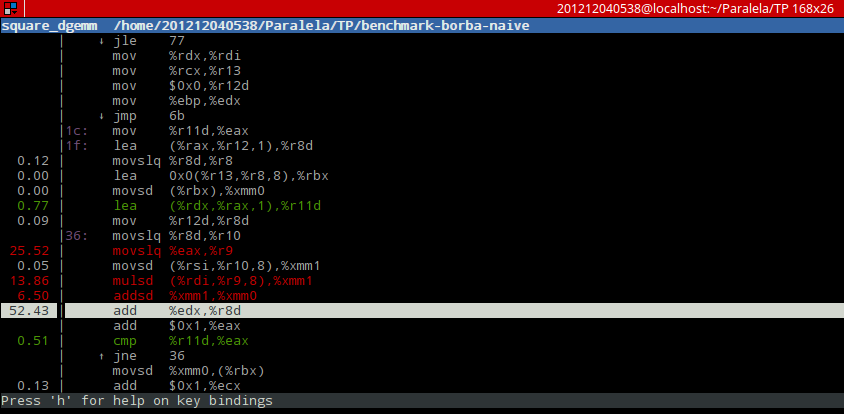
\includegraphics[scale=0.5]{images/perf_ops}
    \end{center}
    \caption{Profiling realizado pelo programa perf no algoritmo modificado, em termos de processamento.}
    \label{fig:perf_ops}
\end{figure}



  
 \section{Resultados Computacionais}
  
Todos os testes aqui descritos foram executados na máquina Katrina, que tem como processador um Intel Haswell-EP de 6 cores (12 threads) executando a 2.4 GHz e Cache de 15 M, resultando em:
\begin{verbatim}
     8 double-precision (64-bit) flops por pipeline * 6 pipelines * 2.4 GHz = 115.2 Gflops/s. (Intel(R) Xeon(R) CPU E5-2620 v3 @ 2.40GHz, (CPU speed in GHz) x (number of CPU cores) x (CPU instruction per cycle) x (number of CPUs per node).) 
\end{verbatim} 
  
  
Para a execução dos testes computacionais foi utilizada a função de benchmark disponibilizada para este mesmo fim. Essa função utiliza um conjunto representativo de tamanhos de matrizes (múltiplos de $32 \pm 1$) para executar a função de multiplicação de matrizes capturando o tempo de execução. A partir das características da máquina, a função calcula o desempenho do programa em Mflops e em porcentagem da capacidade total de processamento da máquina. 
  
\begin{figure}[H]
    \begin{center} 
        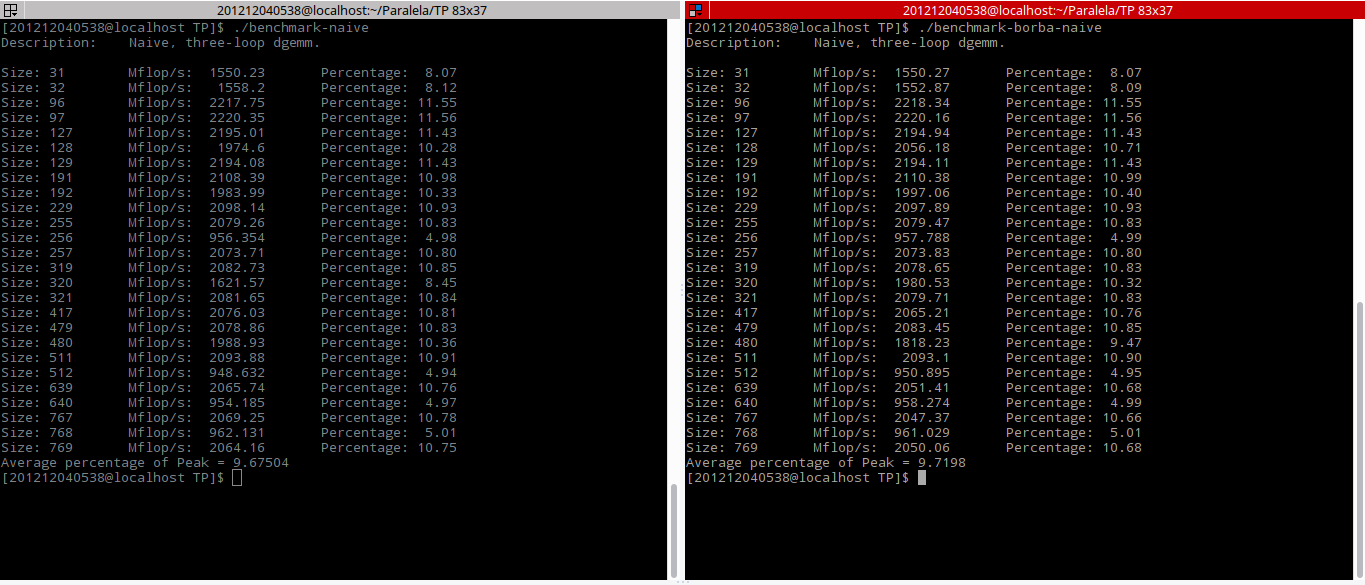
\includegraphics[scale=0.33]{images/exec_comp}
    \end{center}
    \caption{Execução das multiplicações ingênuas de matrizes, original (à esquerda) e modificado (à direita)}
    \label{fig:comp}
\end{figure}

Executando os processos em sequência (para evitar a concorrência), tal como exibido na figura \ref{fig:comp} e comparando unicamente os valores obtidos em MFlops/s foi possível montar dois gráficos, que podem ser vistos nas duas figuras abaixo. O primeiro gráfico compara a porcentagem de uso da capacidade total da CPU do servidor Katrina, enquanto o segundo gráfico explora as diferenças em percentual dos dois algoritmos.


\begin{figure}[H]
    \begin{center} 
        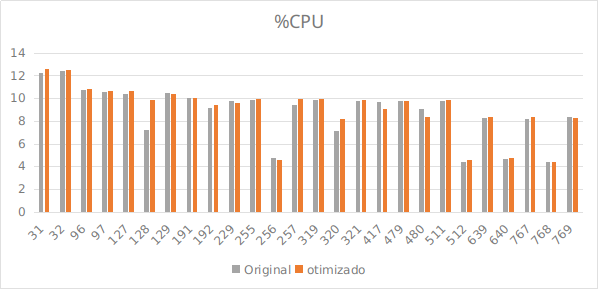
\includegraphics[scale=0.6]{images/grafico2_1}
    \end{center}
    \caption{Rendimento em porcentagem de Capacidade total da CPU para os algoritmos}
    \label{fig:comp}
\end{figure}


\begin{figure}[H]
    \begin{center} 
        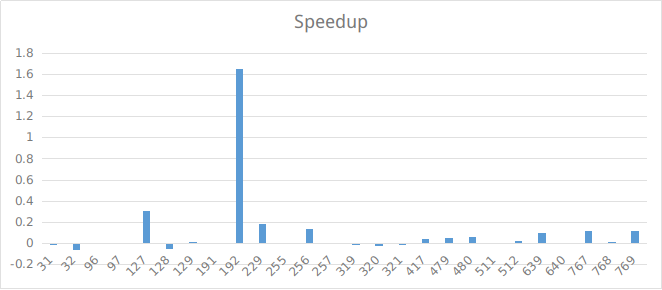
\includegraphics[scale=0.6]{images/speedup_2}
    \end{center}
    \caption{Diferença percentual entre o algoritmo utilizado e o algoritmo}
    \label{fig:comp}
\end{figure}

Percebe-se uma grande otimização para o tamanho de matrizes de 192x192. Esse valor é um divisor do tamanho da cache, o que indica que armazenar o valor mais utilizado em um registrador pode realmente valer a pena: 

$$
     15M = 1024\times15 = 15360.
$$
$$
     \frac{15360}{192} = 80 \text{páginas}
$$

Utilizando a mesma estrutura de testes, agora compara-se o código escrito com otimizações e seu código original compilado com as diretivas \textit{-O3 fstrict-aliasing -std=gnu99}, obtivemos o gráfico da figura \ref{fig:OxB}, que representa o ganho (em porcentagem) da otimização realizada manualmente ante à otimização do compilador.
  

\begin{figure}[H]
    \begin{center} 
        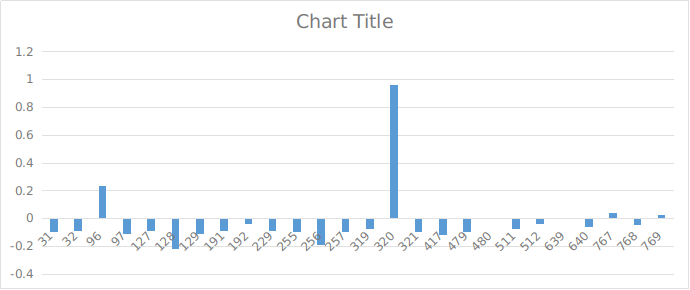
\includegraphics[scale=0.6]{images/O3xBorba}
    \end{center}
    \caption{Resultados do ganho da otimização escrita, em comparação com a realizada pelo compilador}
    \label{fig:OxB}
\end{figure}  

Nota-se que os resultados do otimizador do compilador são ligeiramente melhores (valores negativos) enquanto as otimizações manuais se mostraram mais efetivas nos tamanhos de matrizes 96 e 320 (chegando a 1\% a mais de utilização da capacidade total da CPU). Tal resultado pode ser explicado pelas características do processador (que tem um processador de 3.20 GHz) em conjunto com a otimização da gerência de memória, utilizando um registrador para armazenar o valor mais comumente utilizado, evitando cache misses e aproveitando melhor o tempo para realizar operações de ponto flutuante. 

\section{Conclusão}

As otimizações realizadas foram apenas ligeiramente eficientes, chegando próximas ao otimizador do compilador, mas perdendo um pouco para ele. Estima-se, no entanto, que estas otimizações ajudem a melhorar significantemente o paralelismo que será futuramente feito.

Os próximos passos envolvem Loop Unrolling, e a pesquisa e implementação de um método mais eficiente de multiplicação de matrizes. 

\newpage
\begin{thebibliography}{9}

    \bibitem{bilmes} BILMES, J. Optimizing Matrix Multiply using PHiPAC: a Portable, High-Performance, ANSI C Coding Methodology\\
    Disponível em \textit{https:\/\/people.eecs.berkeley.edu\/\~krste\/papers\/phipac\_ics97.pdf}\\
    Acesso em 2 de Setembro de 2017

\end{thebibliography}



\end{document}


